\chapter{Wprowadzenie teoretyczne}

\section{Geneza historyczna}
Problem swoją nazwę zawdzięcza imperium rzymskiemu. Po raz pierwszy został opisany w artykule ,,Defend Roman Empire!".\cite{defendRomanEmpire}
Obrazuje on problem następująco: Każdy wierzchołek grafu reprezentuje pewną lokalizację (miasto, wzgórze) w Imperium Rzymskim. Lokalizacja (wierzchołek $v$) jest niechroniona, jeśli nie stacjonują w niej żadne legiony wojska ($f(v) = 0$) oraz chroniona jeśli ($f(v) \in {1,2} $). Wartości te oznaczają liczbę legionów stacjonujących w danej lokalizacji. Niechroniona lokalizacja może być ochroniona poprzez wysłanie legionu stacjonującego w lokalizacji sąsiadującej. W czwartym wieku cesarz Konstantyn Wielki wydał dekret zakazujący przemieszczenia się legionu do lokalizacji sąsiadującej, jeśli sprawi to, że aktualna lokalizacja pozostanie niechroniona. Dlatego, żeby móc wysłać legion do sąsiedniej lokacji, w aktualnej muszą stacjonować dwa legiony. Oczywiście, cesarzowi zależało na jak najmniejszych kosztach utrzymywania legionów, a zatem, żeby było ich jak najmniej. \cite{theoryWCRDF} Problem możemy zatem zinterpretować grafowo, gdzie lokalizacje to wierzchołki grafu, liczba legionów to wartości na wierzchołkach. W celu zachowania ciągłości efektywnej komunikacji między legionami wymagana jest słabo spójność zbioru dominującego.

\section{Definicja problemu}
Jako, że problem nie jest powszechnie znany, należy go zdefiniować, wprowadzając następujące pojęcia \cite{theoryWCRDF}:

\newtheorem{definition}{Definicja}

\begin{definition}
    Funkcja dominująca rzymska zdefiniowana jest dla grafu $G = (V, E)$, gdzie $f: V -> \{0,1,2\}$ spełnia warunek, że dla każdego wierzchołka $u$, dla którego $f(u) = 0$ jest sąsiadem przynajmniej jednego wierzchołka $v$, dla którego $f(v) = 2$.
\end{definition}

\begin{definition}
    Dominujący zbiór $D \subseteq V$ jest zbiorem dominującym słabo spójnym grafu $G$ jeśli graf $(V,E \cap (D \times V))$ jest spójny.
\end{definition}

\begin{definition}
    Funkcja dominująca rzymska słabo spójna na grafie $G$ będzie funkcją dominującą rzymską, taką, że zbiór $\{u \in V: f(u) \in \{1,2\}\}$ jest jednocześnie zbiorem dominującym słabo spójnym.
\end{definition}

\begin{definition}
    Wagę funkcji dominującej rzymskiej słabo spójnej definiujemy jako $f(V) = \sum_{u \in V}{f(u)}$. Minimalną wartość tej funkcji nazywamy liczbą dominowania rzymskiego słabo spójnego - $\gamma_{R}^{\text{wc}}(G)$. 
\end{definition}

\begin{definition}
    Jeśli graf $G$ ma następującą własność: $\gamma_{R}^{\text{wc}}(G) = 2\gamma_{\text{wc}}(G)$, to nazywa się go grafem rzymskim słabo spójnym.
\end{definition}

\begin{figure}[H]
    \centering
    \includegraphics[width=0.5\textwidth]{assets/phase2.png}
    \caption{Przykład grafu rzymskiego słabo spójnego.}
    \label{fig:przykladWCRDF}
\end{figure}

Od tego momentu zbiór dominujący rzymski słabo spójny będzie definiowany jako $WCRDS$, funkcja dominowania rzymskiego słabo spójnego to $WCRDF$. Problem dominowania rzymskiego słabo spójnego będzie oznaczany jako $WCRDP$.

\section{Złożoność obliczeniowa}
Poniższy szkic dowodu został przedstawiony w artykule: ,,Weakly connected Roman domination in graphs" \cite{theoryWCRDF}. 
Za pomocą redukcji alfa problem WCRDF zostanie sprowadzony do NP-zupełnego problemu dokładnego pokrycia 3 zbiorami (Exact Cover by 3-Sets, X3C)\cite{X3C}, czym zostanie udowodniona NP-zupełność wersji decyzyjnej WCRDF. Naturalnie, wersja minimalizycjna -  $\gamma_{R}^{\text{wc}}(G)$ jest wtedy NP-trudna.\\
\textbf{Dane:} Spójny graf $G$ oraz dodatnia liczba całkowita $k$.\\
\textbf{Pytanie:} Czy istnieje słabo spójna funkcja dominacji rzymskiej w grafie $G$ o wadze co najwyżej $k$?\\

\textbf{Problem WCRDF jest NP-zupełny, nawet dla grafów podziału (graf, w którym można wydzielić klikę oraz zbiór niezależny) oraz grafów dwudzielnych.}\\

Szkic dowodu:\\
Problem WCRDF należy do klasy NP, ponieważ dla danego przyporządkowania $f : V(G) \rightarrow \{0, 1, 2\}$ można w czasie wielomianowym sprawdzić, czy $f$ ma wagę co najwyżej $k$ oraz czy spełnia warunki WCRDF.

Redukcja jest przeprowadzana z problemu dokładnego pokrycia 3-zbiorami (Exact Cover by 3-Sets, X3C). Dla danej instancji $X = \{x_1, \dots, x_{3q}\}$ i rodziny zbiorów $\mathcal{C} = \{C_1, \dots, C_m\}$, gdzie każdy $C_j \subseteq X$ oraz $|C_j| = 3$, konstruowany jest graf podziału $G$.

Dla każdego elementu $x_i \in X$ oraz zbioru $C_j \in \mathcal{C}$ tworzone są wierzchołki. Dodaje się krawędź między $x_i$ a $C_j$ wtedy i tylko wtedy, gdy $x_i \in C_j$. Dodatkowo wierzchołki odpowiadające zbiorom $C_j$ tworzą klikę $K_m$ (poprzez połączenie tych wierzchołków krawędziami). Przyjęto: $k = 2q$.

Można wykazać, że $\mathcal{C}$ zawiera dokładne pokrycie zbioru $X$ wtedy i tylko wtedy, gdy graf $G$ posiada słabo spójną funkcję dominacji rzymskiej o wadze co najwyżej $k$.\\

Przykładową konstrukcję można zdefiniować następująco:
\begin{align*}
X &= \{x_1, x_2, x_3, x_4, x_5, x_6\} \\
\mathcal{C} &= \left\{
\begin{array}{l}
C_1 = \{x_1, x_2, x_3\}, \\
C_2 = \{x_2, x_4, x_5\}, \\
C_3 = \{x_4, x_5, x_6\}
\end{array}
\right\}
\end{align*}
\begin{align*}
C_1 \cup C_3 &= \{x_1, x_2, x_3, x_4, x_5, x_6\} = X \\
q &= 2 \\
k &= 2q = 4
\end{align*}

Zgodnie z konstrukcją, wierzchołki $x$ zostaną połączone z wierzchołkami $C$, zgodnie z  $x_i \in C_j$. W tym przypadku liczba zbiorów dokładnego pokrycia 3-zbiorami wynosi 2 i są to zbiory $C_1$ oraz $C_2$. Je również należy połączyć krawędzią. Wierzchołki należące do WCRDS to $C_1$ oraz $C_2$. Zgodnie z WCRDF, nadanie im wartości 2 spełnia jego definicję. \\
Poniżej umieszczono rysunek poglądowy (na czerwono wierzchołki należące do WCRDS):

\begin{center}
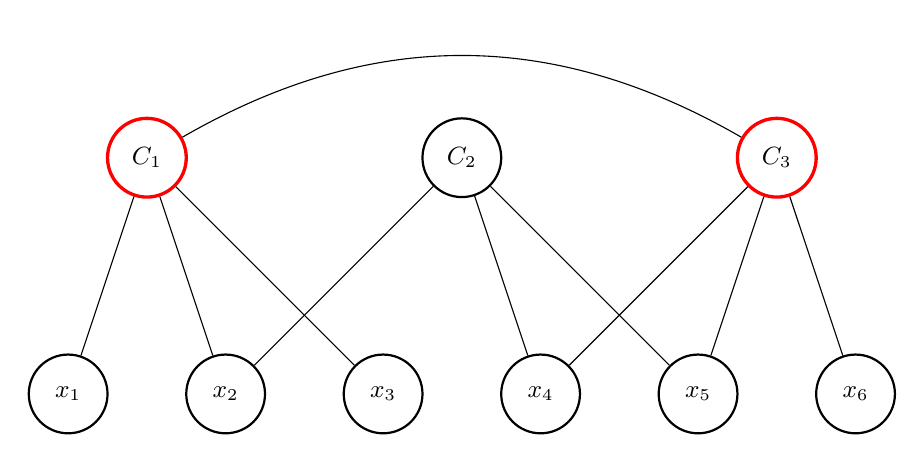
\begin{tikzpicture}[
    vertex/.style={circle,draw,thick,minimum size=1cm},
    redvertex/.style={circle,draw=red,very thick,minimum size=1cm},
    every node/.style={font=\small}
]

% Wierzchołki X (dół)
\node[vertex] (x1) at (0,0) {$x_1$};
\node[vertex] (x2) at (2,0) {$x_2$};
\node[vertex] (x3) at (4,0) {$x_3$};
\node[vertex] (x4) at (6,0) {$x_4$};
\node[vertex] (x5) at (8,0) {$x_5$};
\node[vertex] (x6) at (10,0) {$x_6$};

% Wierzchołki C (góra)
\node[redvertex] (C1) at (1,3) {$C_1$};
\node[vertex] (C2) at (5,3) {$C_2$};
\node[redvertex] (C3) at (9,3) {$C_3$};

% Krawędzie z C do X
\draw (C1) -- (x1);
\draw (C1) -- (x2);
\draw (C1) -- (x3);

\draw (C2) -- (x2);
\draw (C2) -- (x4);
\draw (C2) -- (x5);

\draw (C3) -- (x4);
\draw (C3) -- (x5);
\draw (C3) -- (x6);
\draw (C3) to[bend right] (C1);

\end{tikzpicture}
\end{center}

Aby uzyskać wynik również dla grafów dwudzielnych, naleźy zmodyfikować konstrukcję: zamiast dodawać krawędzie między wierzchołkami $C_j$, dodajemy cztery nowe wierzchołki $y_0, y_1, y_2, y_3$ oraz krawędzie $y_0y_1$, $y_0y_2$, $y_0y_3$ i $y_0C_j$ dla każdego $j$. Ustawiamy wtedy $k = 2q + 2$.\\

Konstrukcję dla przykładowego grafu dwudzielnego przedstawia poniższy rysunek. k będzie wynosiło 6.\\

\begin{center}
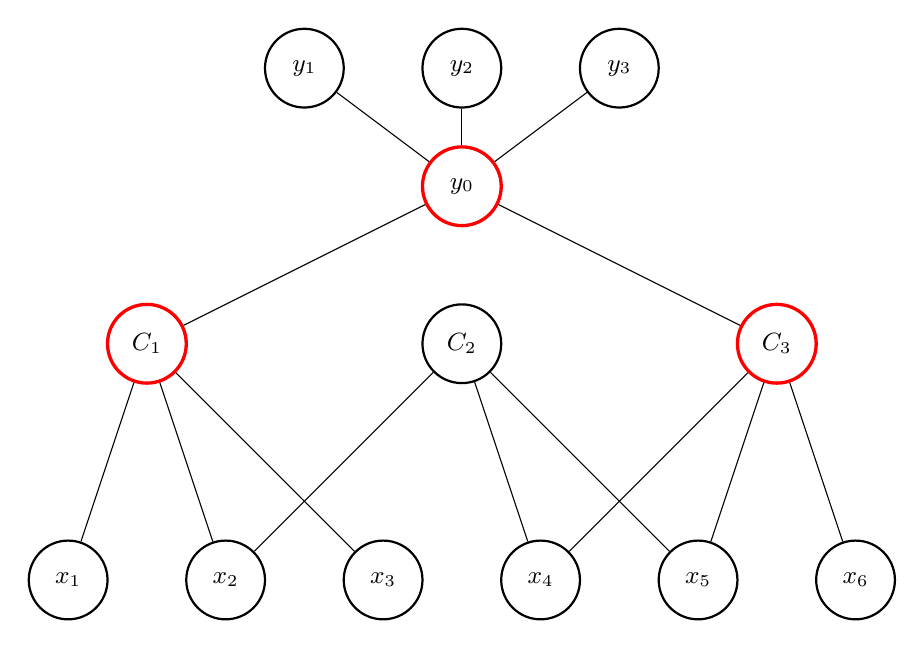
\begin{tikzpicture}[
    vertex/.style={circle,draw,thick,minimum size=1cm},
    redvertex/.style={circle,draw=red,very thick,minimum size=1cm},
    every node/.style={font=\small}
]

% Wierzchołki X (dół)
\node[vertex] (x1) at (0,0) {$x_1$};
\node[vertex] (x2) at (2,0) {$x_2$};
\node[vertex] (x3) at (4,0) {$x_3$};
\node[vertex] (x4) at (6,0) {$x_4$};
\node[vertex] (x5) at (8,0) {$x_5$};
\node[vertex] (x6) at (10,0) {$x_6$};

% Wierzchołki C (góra)
\node[redvertex] (C1) at (1,3) {$C_1$};
\node[vertex] (C2) at (5,3) {$C_2$};
\node[redvertex] (C3) at (9,3) {$C_3$};

% Wierzchołek pośredni i łączniki
\node[redvertex] (y0) at (5,5) {$y_0$};
\node[vertex] (y1) at (3,6.5) {$y_1$};
\node[vertex] (y2) at (5,6.5) {$y_2$};
\node[vertex] (y3) at (7,6.5) {$y_3$};

% Krawędzie z C do X
\draw (C1) -- (x1);
\draw (C1) -- (x2);
\draw (C1) -- (x3);

\draw (C2) -- (x2);
\draw (C2) -- (x4);
\draw (C2) -- (x5);

\draw (C3) -- (x4);
\draw (C3) -- (x5);
\draw (C3) -- (x6);

% Krawędzie od y0 do C
\draw (y0) -- (C1);
\draw (y0) -- (C3);

% Krawędzie y0-y1/y2/y3
\draw (y0) -- (y1);
\draw (y0) -- (y2);
\draw (y0) -- (y3);

\end{tikzpicture}
\end{center}

\section{Przegląd literatury}
W 2004 roku zdefiniowano formalnie funkcję dominowania rzymskiego (RDF) \cite{RDF} i od tego czasu w wielu publikacjach analizowano właściwości tego parametru oraz inne wersje dominowania rzymskiego, m.in. silna, mieszana, totalna dominacja rzymska.\\ 
Henning i Hedetniemi w 2003 roku udowodnili, że problem słabego dominowania rzymskiego jest NP-zupełny w wersji decyzyjnej, nawet dla grafów dwudzielnych. \cite{NEW_STRATEGY} \\ 
W artykule z 2019 roku wprowadzono pojęcie słabo spójnego dominowania rzymskiego. Zdefiniowano WCRDF oraz $\gamma_{R}^{\text{wc}}(G)$ oraz następujące właściwości:
\begin{itemize}
    \item Dla każdego spójnego grafu $G$ zachodzi:
    \[
    \gamma_{\text{wc}}(G) \leq \gamma_{R}^{\text{wc}}(G) \leq 2\gamma_{\text{wc}}(G)
    \]
    co oznacza, że liczba słabo spójnej dominacji rzymskiej jest ograniczona od dołu przez klasyczną liczbę słabo spójnej dominacji oraz od góry przez jej podwojenie.

    \item Dla spójnego grafu $G$, $\gamma_{\text{wc}}(G) = \gamma_{R}^{\text{wc}}(G)$ zachodzi wtedy i tylko wtedy, gdy $G = K_1$ (graf jednoelementowy).

    \item Dla dowolnego spójnego grafu $G$ o $n$ wierzchołkach:
    \[
    \gamma_{R}^{\text{wc}}(G) \leq n
    \]
    z równością wtedy i tylko wtedy, gdy $G \in \{K_1, K_2\}$.

    \item Jeżeli $\gamma_{R}^{\text{wc}}(G) < n$ oraz $f = (V_0, V_1, V_2)$ jest funkcją minimalną WCRDF, to zachodzi:
    \[
    |V_0| > 0 \quad \text{oraz} \quad |V_2| > 0
    \]
    czyli co najmniej jeden wierzchołek musi mieć wartość 0, a co najmniej jeden wartość 2.
\end{itemize}
Dodatkowo pokazano, że problem ten jest NP-zupełny, nawet dla grafów dwudzielnych \cite{theoryWCRDF}.\\
W 2021 rozszerzono wiedzę z poprzedniej publikacji o charakteryzację słabo spójnych drzew rzymskich oraz pokazano, że sprawdzenie, czy graf dwudzielny jest rzymski słabo spójny jest co-NP-trudne \cite{PROGRESS}.\\
W 2021 roku Chakradhar i współautorzy zaproponowali dwa nowe modele programowania liniowego całkowitoliczbowego oraz algorytm $2(1+\epsilon)(1 + \ln(\Delta - 1))$-aproksymacyjny. W ramach niniejszej pracy, analizowane będą te dwa modele programowania liniowego oraz aproksymacyjny \cite{ILP}.\\
Dodatkowo analizowane będą propozycje własne rozwiązania tego problemu.
W 2023 roku ukazal się artykuł proponujący GRASP (Greedy Randomized Adaptive Search Procedure) - zachłanna losowa procedura adaptacyjnego przeszukiwania dla problemu znajdowania $\gamma_{R}^{\text{wc}}(G)$, poprzez zdefiniowanie funkcji zachłannych: Dscore (dominacja) i Nscore (sąsiedztwo), strategie tabu w celu uniknięcia zapetlenia oraz lokalnych przeszukiwań w celu optymalizacji rozwiązania. Jednakże, autorzy artykułu źle zrozumieli definicję WCRDS, dlatego jego wyniki nie zostały dalej analizowane \cite{GRASP}.
Literatura proponuje również zastosowanie rozwiązania tego problemu w obecnych czasach. Mianowicie, kosztowne pojazdy służb ratunkowych powinny być rozmieszczane tak, aby były w stanie udzielić pomocy potrzebującym, przy możliwie dużej redukcji kosztów utrzymania takiego pojazdu. Dlatego, na wzór legionów rzymskich, w budynkach służb ratunkowych powinien znajdować się pojazd, bądź być możliwość wypożyczenia go z sąsiedniej (najbliższej) lokalizacji służb ratunkowych \cite{improvedILP}.

\section{Metody badań}
W celu implementacji i testowania wydajności oraz poprawności algorytmów, stworzono program w języku Python, ze wsparciem następujących bibliotek:
\begin{itemize}
    \item networkx - pakiet dostarczający funkcje umożliwiające operacje na grafach, wykresach i sieciach
    \item matplotlib - do wyświetlania wyników działania algorytmów w postaci wykresów grafów
    \item time - wykorzystywane do pomiarów czasu pracy algorytmów
    \item pulp - do programowania liniowego
    \item pandas - do analizy danych z csv
    \item geopandas - do analizy współrzędnych geograficznych
    \item itertools - do zagadnień kombinatorycznych
\end{itemize}

Program umożliwia wprowadzenie dowolnego grafu w postaci listy wierzchołków oraz krawędzi, jak i wygenerowanie losowego grafu. Następnie wybrane algorytmy analizują dany graf poprzez przypisywanie odpowiednich wartości wierzchołkom oraz wyliczania liczby dominowania rzymskiego słabo spójnego. Dla każdego z algorytmów wyliczany i zapisywany jest ich czas działania. Na końcu program wyświetla wykres z nadanymi wartościami na wierzchołkach.\\

W celu przeprowadzenia testów wygenerowano oraz zapisano w plikach grafy następujących klas: 
\begin{itemize}
    \item gęste - \textit{nx.erdos\_renyi\_graph(p=0.7)} - z racji wielu krawędzi, co może znacznie wpłynąć na wyniki osiągane przez algorytmy, gdzie p to prawdopodobieństwo wystąpienia krawędzi,
    \item rzadkie - \textit{nx.erdos\_renyi\_graph(p=0.3)} - z racji mniejszej liczby krawędzi, w celu zweryfikowania hipotezy, że dla tych grafów algorytmy będą działały szybciej,
    \item drzewa - \textit{nx.random\_unlabeled\_rooted\_tree(n)} - z racji implementacji specjalnego liniowego algorytmu dla drzew, który znajduje $\gamma_{R}^{\text{wc}}(G)$ oraz specyficznych własności drzew,
    \item bezskalowe - \textit{nx.barabasi\_albert\_graph()} - grafy nieregularne, z powodu hipotetycznych zastosowań praktycznych, dobrze odzwierciedlają naturalnie powstające na świecie grafy np. sieci społecznościowych, komputerowych, energetycznych.
\end{itemize}

Grafy te wygenerowano kilka razy dla konkretnej liczby wierzchołków. Liczby wierzchołków, dla których przeprowadzano analizę to $[10, 20, 30, 40, 50]$. Wszystkie algorytmy zostały użyte dla tego samego zestawu grafów, w celu zachowania miarodajności przy analizie porównawczej. Wszystkie wyniki działania algorytmów na wszystkich wygenerowanych przykładowych grafach zostały zapisane w pliku csv. Zapisano tam również pomiary czasu oraz WCRDF oraz wyznaczoną $\gamma_{R}^{\text{wc}}(G)$. Dodatkowo zapisano też wykresy grafów wraz z przypisanymi wartościami WCRDF.\\

Czas mierzono za pomocą funkcji \textit{time.perf\_counter\_ns()}, dając wyniki w nanosekundach o dokładności pomiaru 100 [ns]. Wyniki pomiaru czasu działania są uśrednione, wykonywane pięciokrotnie, aby uniknąć niespodziewanych odchyleń.\\

Przeprowadzono również dostosowywanie parametrów dla algorytmu mrówkowego na wcześniej wygenerowanych grafach, w celu znalezienia jak najlepszych parametrów dla tego konkretnego problemu. Nastepnie, na podstawie wielkości błędu dokonano wyboru najlepszego zestawu parametrów, których używano później w docelowej analizie porównawczej.\\

Algorytmy wyznaczjące poprawnie WCRDF, jednakże nie zawsze wyznaczjące $\gamma_{R}^{\text{wc}}(G)$, poddano dodatkowej analizie w celu określenia rozbieżności od optymalnego wyniku.

Następnie algorytmy zostały poddane analizie na grafach naturalnie powstałych.\\

Dzięki bibliotece geopandas utworzono mapę Polski, a nastepnie naniesiono na niej punkty odpowiadające węzłom przesyłowym sieci najwyższych napięć w Polsce, na podstawie istniejącego w Polsce planu. Na grafie starano się odwzorować najważniejsze punkty i krawędzie tej sieci przesyłowej. Z tych danych powstał graf, który następnie zbadano przy użyciu zaimplementowanych algorytmów. Rozmieszczenie wartości WCRDF ma odpowiadać lokalizacjom mechanizmów zabezpieczających sieć przesyłową w razie awarii jednej ze stacji \cite{POLAND}.\\

Następnie analizowano naturalne grafy odzwierciedlające sieci społecznościowe. Są to: mały graf sieci klubu karate Zacharego z 34 wierzchołkami i 78 krawędziami \cite{KARATE}, oraz graf dużej sieci społecznościowej znajomych z Facebook'a (4039 wierzchołki i 80234 krawędzi) \cite{FACEBOOK}. W przypadku sieci społecznościowych WCRDF może mieć zastosowanie w optymalnym rozmieszczeniu agentów wykrywających oszustwa w internetowej sieci społecznościowej.\\

Dla grafów naturalnie powstałych również mierzono czas działania, jak i jakość prezentowanych przez algorytmy wyników.



